\section{An independent anatomical ground truth}

The synthetic instrument of \S\ref{sec:synthetic-instrument} answers whether
the pipeline can recover a correspondence it generated itself. It cannot, by
construction, answer whether the pipeline is right about a \emph{real}
specimen. Closing that gap required an independent reference the pipeline
had no part in producing.

\begin{figure}[!htb]
\centering
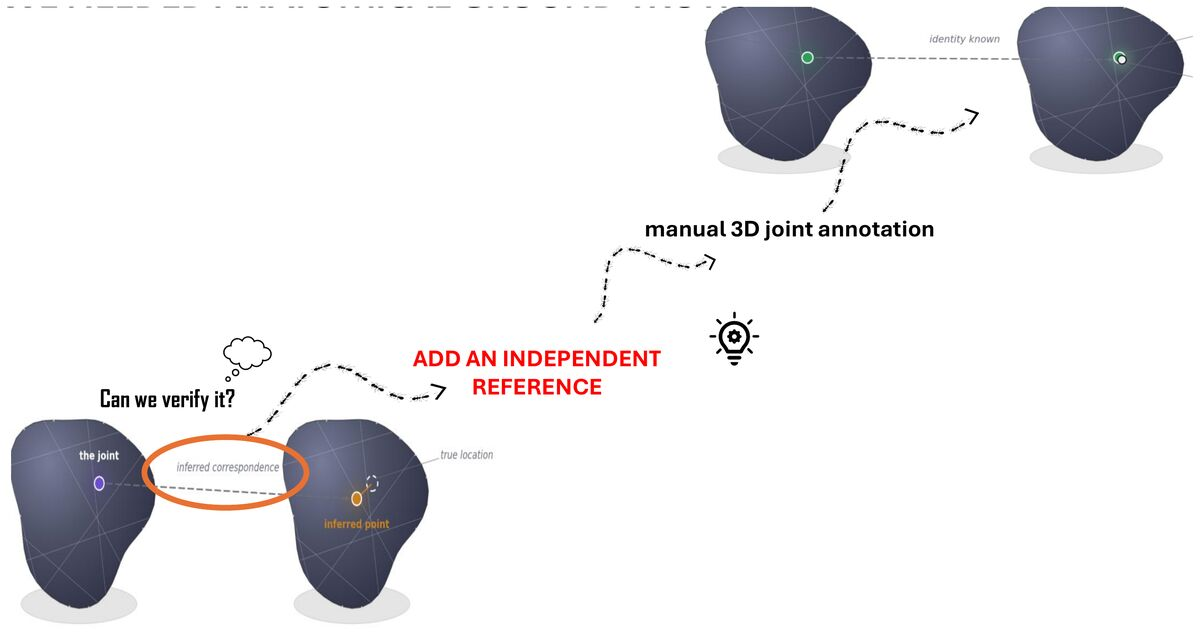
\includegraphics[width=0.55\linewidth]{figures/fig_ground_truth_annotation.jpg}
\caption{Manual 3D joint annotation as an independent reference: an expert
places joints directly on the scan, with identity known by construction,
against which the model's inferred correspondence can be verified rather
than merely inspected.}
\label{fig:ground-truth-annotation}
\end{figure}

\begin{figure}[!htb]
\centering
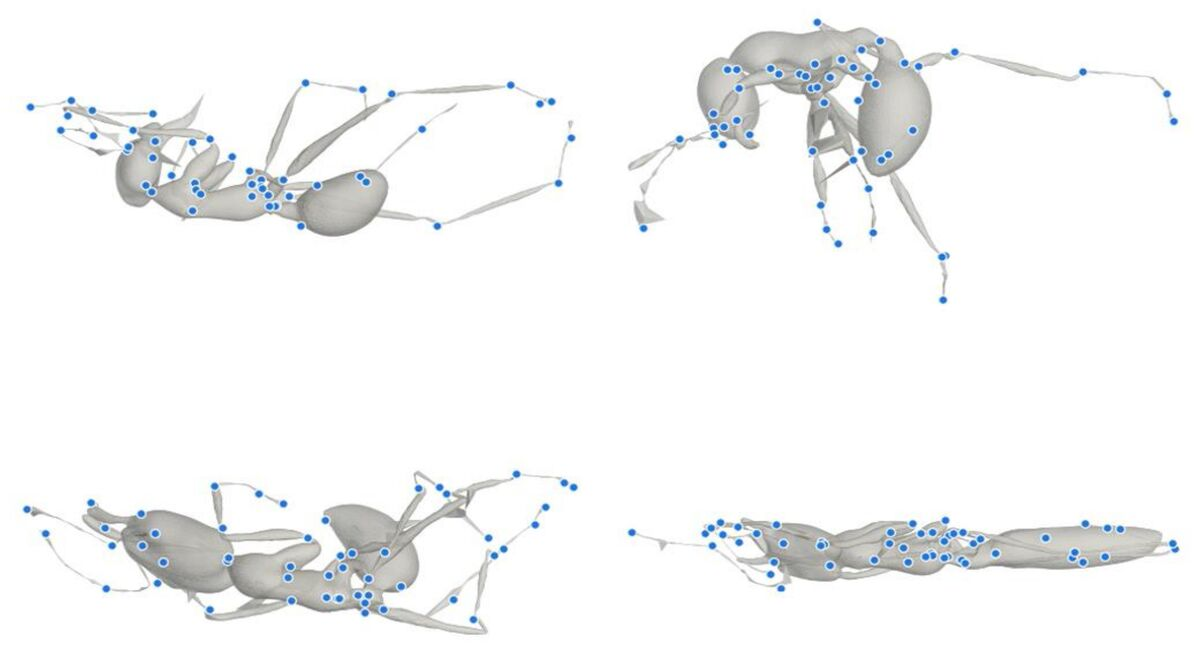
\includegraphics[width=0.6\linewidth]{figures/fig_landmarks_structured.jpg}
\caption{Expert-annotated joints across four specimens. Reliability is not
uniform across the body: it is structured, concentrated proximally, and
degrades toward the distal leg and antenna segments, consistent with the
sampling deficit in \F{F5}.}
\label{fig:landmarks-structured}
\end{figure}

Manual 3D joint annotation (Figure~\ref{fig:ground-truth-annotation})
supplies this reference. Evaluated against it, the delivered fits are close
to unbiased across every anatomical block, but, as \S\ref{sec:reliability}
details, do not reliably \emph{rank} specimens against one another. This
is the first accuracy statement in the project grounded in expert-verified
data rather than the pipeline's own synthetic ground truth, and it is not
uniformly favourable: it delimits precisely which claims the current fits
support (Figure~\ref{fig:landmarks-structured}).
